\documentclass[11pt,a4paper]{article}

% ---- Idioma y tipografía
\usepackage[spanish, es-noquoting, es-noshorthands]{babel}
\usepackage[T1]{fontenc}
\usepackage[utf8]{inputenc} % eliminar si usas XeLaTeX/LuaLaTeX
\usepackage{lmodern}
\usepackage{microtype}

% ---- Matemáticas
\usepackage{amsmath}
\usepackage{amssymb}

% ---- Márgenes y diseño
\usepackage[a4paper,margin=2.5cm]{geometry}
\usepackage{parskip}

% ---- Enlaces
\usepackage[hidelinks]{hyperref}
\usepackage{bookmark}

% ---- Cabeceras y pies
\usepackage{fancyhdr}
\pagestyle{fancy}
\fancyhf{}
\renewcommand{\headrulewidth}{0.4pt}
\lhead{\textsc{\asignatura}}
\rhead{\textbf{\tema}}
\cfoot{\thepage}

% ---- Listas y símbolos
\usepackage{enumitem}
\setlist{itemsep=0.3em, topsep=0.5em}

% ---- Iconos y color
\usepackage{fontawesome5}
\usepackage{xcolor}
\usepackage[most]{tcolorbox}
\tcbuselibrary{breakable,skins}

% ---- Figuras
\usepackage{graphicx}
\usepackage{caption}

% ---- Colores propios
\definecolor{uniPrimary}{HTML}{0A7AC3}
\definecolor{uniSoft}{HTML}{E9F4FB}
\definecolor{uniAccent}{HTML}{F5B700}
\definecolor{uniOK}{HTML}{2E7D32}
\definecolor{uniWarn}{HTML}{C62828}

% ---- Metadatos reutilizables
\newcommand{\asignatura}{Seguridad de Sistemas Informáticos}
\newcommand{\tema}{Tema 2 — Criptografía}
\newcommand{\clase}{Clase 1}

% ---- Estética de secciones
\usepackage{titlesec}
\titleformat{\section}{\Large\bfseries\color{uniPrimary}}{\thesection}{0.6em}{}
\titleformat{\subsection}{\large\bfseries}{\thesubsection}{0.5em}{}
\titleformat{\subsubsection}{\bfseries}{\thesubsubsection}{0.5em}{}

% ---- Cajas reutilizables
\tcbset{
    commonstyle/.style={
        enhanced, breakable,
        left=8pt,right=8pt,top=8pt,bottom=8pt,
        boxrule=0.8pt,
        fonttitle=\bfseries
    }
}

\newtcolorbox{ObjetivosBox}[1][]{
    commonstyle,
    title={\faBullseye\; Índice},
    colback=uniSoft, colframe=uniPrimary,#1
}

\newtcolorbox{DefBox}[1][]{
    commonstyle,
    title={\faBook\; Definición},
    colback=white, colframe=uniAccent,#1
}

\newtcolorbox{NotaBox}[1][]{
    commonstyle,
    title={\faStickyNote\; Nota},
    colback=white, colframe=uniPrimary,#1
}

\newtcolorbox{RecordatorioBox}[1][]{
    commonstyle,
    title={\faBell\; Recordatorio},
    colback=uniAccent!15, colframe=uniAccent,#1
}

\newtcolorbox{ChecklistBox}[1][]{
    commonstyle,
    title={\faTasks\; Tareas / Checklist},
    colback=white, colframe=uniPrimary,#1
}

\newtcolorbox{ResumenBox}[1][]{
    commonstyle,
    title={\faHighlighter\; Resumen rápido (5 líneas)},
    colback=uniSoft, colframe=uniPrimary,#1
}

\newtcolorbox{VocabBox}[1][]{
    commonstyle,
    title={\faLanguage\; Vocabulario clave},
    colback=white, colframe=uniPrimary,#1
}

% =========================================================
\begin{document}

\begin{center}
    {\LARGE \textbf{\asignatura}}\\[0.3cm]
    {\large \tema}\\[0.2cm]
\end{center}
\hrule
\vspace{1em}

\tableofcontents

\section{Algoritmos de cifrado}
\subsection{Autenticación de los mensajes}

\begin{DefBox}
La \textbf{autenticación de mensajes} no siempre requiere confidencialidad.
A veces interesa garantizar la autenticidad sin necesidad de ocultar el contenido, como ocurre en documentos de escritura pública.
\end{DefBox}

\begin{NotaBox}
El cifrado por sí solo \textbf{no proporciona autenticación}.
Es posible combinar cifrado y autenticación (por ejemplo, con el algoritmo OCB).
\end{NotaBox}

Normalmente, la autenticación se implementa de forma independiente al cifrado, mediante funciones hash.

\subsubsection*{Autenticación de mensajes con MAC}
\begin{center}
    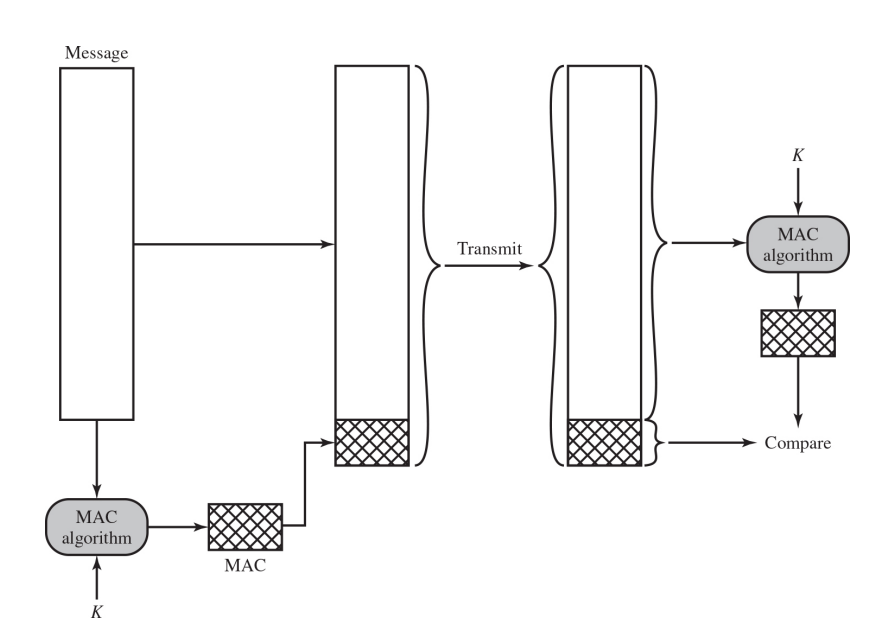
\includegraphics[width=0.6\textwidth]{resources/MAC.png}
    \captionof{figure}{Esquema de autenticación de mensajes con MAC}
\end{center}

\subsubsection*{Autenticación de mensajes con funciones hash unidireccionales}
\begin{center}
    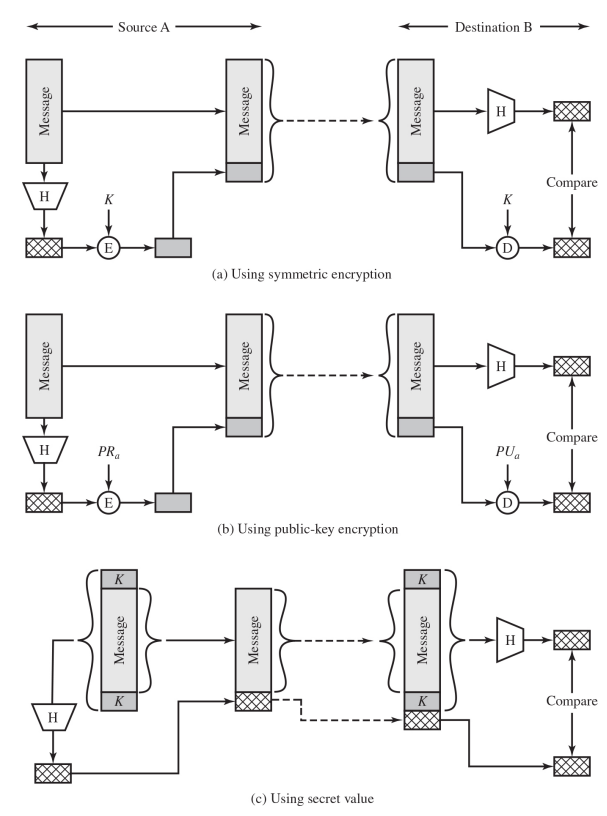
\includegraphics[width=0.6\textwidth]{resources/Hash_Unidirectional.png}
    \captionof{figure}{Esquema de autenticación con funciones hash unidireccionales}
\end{center}

El primer caso es cifrado simétrico, el segundo es cifrado asimétrico. El tercero es usando valor secreto.

\begin{RecordatorioBox}
En este caso no se habla de una “clave” como tal, sino de un \textbf{valor secreto}.
Sólo se denomina clave cuando tanto emisor como receptor deben conocerla.
\end{RecordatorioBox}

\subsection{Criterios de utilidad de una función hash}

Una función hash criptográfica debe cumplir las siguientes propiedades:

\begin{itemize}
    \item \textbf{Entrada arbitraria:} se puede aplicar sobre un conjunto de datos de cualquier tamaño.
    \item \textbf{Determinismo:} para una misma entrada $x$, siempre devuelve el mismo valor $H(x)$.
    \item \textbf{Eficiencia computacional:} $H(x)$ debe calcularse de manera rápida y con un coste razonable.
    \item \textbf{Resistencia a colisiones:} debe ser computacionalmente inviable encontrar dos entradas distintas $x$ y $y$ tales que $H(x)=H(y)$.
    \item \textbf{Irreversibilidad:} dado un valor $h$, debe ser difícil obtener la entrada original $x$ tal que $H(x)=h$.
\end{itemize}

\subsection{Seguridad de las funciones hash}

Existen dos enfoques principales para atacar la seguridad de una función hash:

\begin{itemize}
    \item \textbf{Criptoanálisis:} se centra en explotar debilidades matemáticas o estructurales del algoritmo.
    \item \textbf{Fuerza bruta:} consiste en probar todas las combinaciones posibles. La viabilidad depende de la longitud del código hash generado por el algoritmo.
\end{itemize}

Actualmente, los algoritmos de la familia \textbf{SHA} son los más utilizados en aplicaciones prácticas.

\subsubsection*{Aplicaciones de una función hash segura}

\begin{itemize}
    \item \textbf{Almacenamiento de contraseñas:} en lugar de guardar la contraseña en texto plano, los sistemas almacenan únicamente su valor hash.
    \item \textbf{Integridad de datos:} permite verificar si un archivo o mensaje ha sido modificado. También se aplica en la detección de intrusiones en sistemas.
\end{itemize}

\subsection{Secure Hash Algorithm (SHA)}

El \textbf{Secure Hash Algorithm (SHA)} fue desarrollado originalmente por el \textbf{NIST (National Institute of Standards and Technology)}.
Existen varias versiones de SHA, cada una con distintos parámetros y niveles de seguridad:

\begin{table}[h!]
\centering
\renewcommand{\arraystretch}{1.2}
\setlength{\tabcolsep}{8pt}
\begin{tabular}{|l|c|c|c|c|c|c|c|}
\hline
 & \textbf{SHA-1} & \textbf{SHA-224} & \textbf{SHA-256} & \textbf{SHA-384} & \textbf{SHA-512} & \textbf{SHA-512/224} & \textbf{SHA-512/256} \\ \hline
\textbf{Message size} & $< 2^{64}$ & $< 2^{64}$ & $< 2^{64}$ & $< 2^{128}$ & $< 2^{128}$ & $< 2^{128}$ & $< 2^{128}$ \\ \hline
\textbf{Word size} & 32 & 32 & 32 & 64 & 64 & 64 & 64 \\ \hline
\textbf{Block size} & 512 & 512 & 512 & 1024 & 1024 & 1024 & 1024 \\ \hline
\textbf{Message digest size} & 160 & 224 & 256 & 384 & 512 & 224 & 256 \\ \hline
\textbf{Number of steps} & 80 & 64 & 64 & 80 & 80 & 80 & 80 \\ \hline
\textbf{Security} & 80 & 112 & 128 & 192 & 256 & 112 & 128 \\ \hline
\end{tabular}
\caption{Comparativa de las variantes de SHA}
\end{table}


\begin{NotaBox}
El algoritmo \textbf{SHA-1} ya no se considera seguro, debido a que es vulnerable a ataques de colisión, como el \textit{ataque de cumpleaños}.
\end{NotaBox}

\begin{DefBox}
\textbf{SHA-3} representa un cambio importante en la estructura interna, ya que no se basa en el mismo diseño de SHA-1 y SHA-2.
Permite longitudes de valores hash de 224, 256, 384 y 512 bits.
Una característica clave es que puede aplicarse de forma incremental sobre bloques de datos, sin necesidad de disponer del mensaje completo desde el inicio.
\end{DefBox}

\subsection{Hashed Message Authentication Code (HMAC)}

El \textbf{HMAC} se utiliza en protocolos de seguridad como \textbf{TLS (Transport Layer Security)} o \textbf{SET (Secure Electronic Transaction)}.
Es el estándar de autenticación en muchos protocolos seguros de Internet.

\subsection*{Objetivos de diseño}
\begin{itemize}
    \item Reutilizar funciones hash criptográficas existentes.
    \item Permitir el uso de claves de longitud variable.
    \item Ofrecer un nivel de seguridad equivalente al de la función hash subyacente.
\end{itemize}

\begin{DefBox}
La seguridad de HMAC depende tanto de la \textbf{robustez criptográfica} de la función hash utilizada como de la \textbf{longitud y calidad de la clave secreta}.
Con las funciones y longitudes de clave recomendadas en la actualidad, HMAC se considera seguro.
\end{DefBox}

\subsection{OCB (Offset Codebook Mode)}

El modo \textbf{OCB} es un esquema avanzado que combina en una sola operación dos objetivos fundamentales:
\begin{itemize}
    \item \textbf{Cifrado de la información.}
    \item \textbf{Autenticación del mensaje.}
\end{itemize}

\begin{NotaBox}
Una ventaja de OCB es que el usuario no necesita conocer en detalle su funcionamiento interno para aprovechar sus beneficios de seguridad y eficiencia.
\end{NotaBox}

\subsection{Distribución de claves}

La \textbf{gestión y distribución de claves} es uno de los principales retos en criptografía, ya que debe garantizarse que las claves se compartan de forma segura entre las partes legítimas sin ser interceptadas por terceros.

Algunas estrategias de distribución son:

\begin{itemize}
    \item El emisor (\textbf{A}) entrega físicamente la clave al receptor (\textbf{B}).
    \item Un tercero de confianza selecciona la clave y la distribuye físicamente a ambas partes.
    \item Si \textbf{A} y \textbf{B} ya comparten una clave previa, pueden generar una nueva y enviarla cifrada con la clave antigua.
    \item Si ambos tienen una conexión segura con un tercero (\textbf{C}), este puede generar una clave y distribuirla cifrada a las dos partes.
\end{itemize}

\begin{RecordatorioBox}
El diseño de sistemas criptográficos robustos no solo depende de algoritmos fuertes, sino también de una correcta \textbf{gestión del ciclo de vida de las claves}.
\end{RecordatorioBox}

\subsection*{Requisitos de los criptosistemas de clave pública}

\begin{itemize}
    \item Debe ser \textbf{computacionalmente fácil} generar los pares de claves (pública y privada).
    \item Debe ser \textbf{computacionalmente fácil} para el remitente cifrar mensajes utilizando la \textbf{clave pública} del receptor.
    \item Debe ser \textbf{computacionalmente fácil} para el receptor descifrar los mensajes utilizando su \textbf{clave privada}.
    \item Debe ser \textbf{computacionalmente inviable} para un atacante deducir la \textbf{clave privada} a partir de la \textbf{clave pública}.
    \item Debe ser \textbf{computacionalmente inviable} para un atacante descifrar mensajes cifrados con la \textbf{clave pública} sin conocer la \textbf{clave privada}.
\end{itemize}

\section{Algoritmos de cifrado asimétrico}

Los criptosistemas de clave pública utilizan distintos algoritmos para el cifrado, la firma digital o el intercambio de claves. A continuación, se describen los principales algoritmos asimétricos:

\begin{itemize}
    \item \textbf{RSA (1977):}
    Basado en la factorización de números primos grandes. Es uno de los algoritmos más utilizados en la actualidad para cifrado y firma digital.
    Por razones de seguridad, no se recomienda el uso de claves menores a \textbf{2048 bits}.

    \item \textbf{Diffie--Hellman (1976):}
    Diseñado específicamente para el \textbf{intercambio seguro de claves} a través de un canal inseguro.
    No se utiliza directamente para cifrar o firmar mensajes.

    \item \textbf{DSS (Digital Signature Standard, 1991):}
    Proporciona únicamente una función de \textbf{firma digital}, normalmente implementada junto con el algoritmo \textbf{SHA} (Secure Hash Algorithm).
    No se puede utilizar para cifrado ni para intercambio de claves.

    \item \textbf{Criptografía de Curva Elíptica (ECC, 1985):}
    Basada en la estructura algebraica de las \textbf{curvas elípticas} sobre campos finitos.
    Ofrece el mismo nivel de seguridad que RSA, pero con \textbf{claves de menor tamaño}, lo que mejora el rendimiento y reduce el consumo de recursos.
\end{itemize}

\begin{table}[h!]
\centering
\begin{tabular}{|l|c|c|c|}
\hline
\textbf{Algoritmo} & \textbf{Firma digital} & \textbf{Distribución de claves simétricas} & \textbf{Cifrado de claves secretas} \\ \hline
RSA & Sí & Sí & Sí \\ \hline
Diffie--Hellman & No & Sí & No \\ \hline
DSS & Sí & No & No \\ \hline
Curva elíptica & Sí & Sí & Sí \\ \hline
\end{tabular}
\caption{Comparación de algoritmos de criptografía de clave pública.}
\label{tab:algoritmos_cripto}
\end{table}

\begin{NotaBox}
El algoritmo de \textbf{curva elíptica} utilizado para la firma digital es el \textbf{ECDSA} (\emph{Elliptic Curve Digital Signature Algorithm}).
Para el \textbf{cifrado de claves} se emplea \textbf{ECC} (\emph{Elliptic Curve Cryptography}), y para el \textbf{intercambio de claves}, el algoritmo \textbf{ECDH} (\emph{Elliptic Curve Diffie--Hellman}).
\end{NotaBox}


\subsection{RSA}

El algoritmo \textbf{RSA} (Rivest–Shamir–Adleman) es uno de los sistemas de cifrado asimétrico más utilizados.
Su seguridad se basa en la dificultad de factorizar números compuestos grandes.

\begin{itemize}
    \item \textbf{Cifrado:}
    \[
    C = M^e \bmod n
    \]
    donde \( M \) es el mensaje en claro, \( e \) es el exponente público y \( n \) es el módulo.

    \item \textbf{Descifrado:}
    \[
    M = C^d \bmod n
    \]
    donde \( C \) es el texto cifrado, \( d \) es el exponente privado y \( n \) es el mismo módulo.
\end{itemize}

Tanto el \textbf{emisor} como el \textbf{receptor} deben conocer el valor de \( n \) y \( e \).

\[
\text{Clave pública (PU)} = (e, n)
\]
\[
\text{Clave privada (PR)} = (d, n)
\]

\begin{center}
    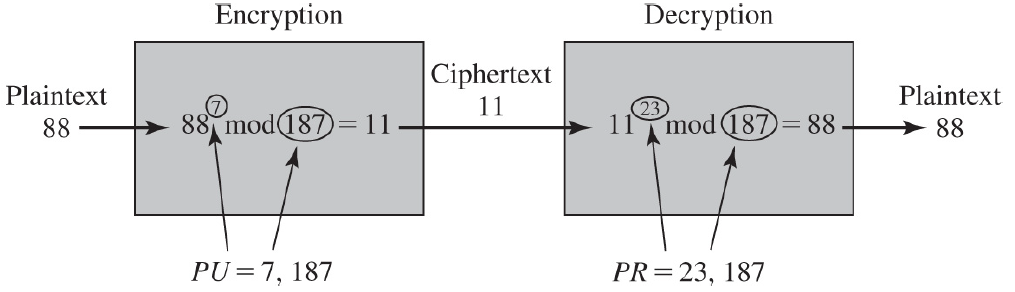
\includegraphics[width=1\textwidth]{resources/RSA_Encryption_Decryption.png}
    \captionof{figure}{Esquema de cifrado y descifrado en RSA}
\end{center}

\subsubsection*{Seguridad de RSA}

\begin{itemize}
    \item \textbf{Fuerza bruta:} implica probar todas las claves privadas posibles.
    \item \textbf{Ataques matemáticos:} basados en la factorización del producto de dos primos grandes.
    \item \textbf{Ataques de tiempo:} Dependen del tiempo de ejecución del algoritmo de descifrado.
    \item \textbf{Ataques de texto cifrado elegido:} explotan propiedades del algoritmo RSA.
\end{itemize}

\begin{NotaBox}
\textbf{Ataques de sincronización.} Un fisgón puede determinar una clave privada midiendo cuánto tiempo tarda una computadora en descifrar un mensaje. No solo son aplicables a RSA, sino también a otros sistemas de cifrado de clave pública.
\end{NotaBox}

\subsection{Intercambio de claves Diffie--Hellman}

Primer algoritmo de \textbf{clave pública} publicado.
Proporciona un método práctico para \textbf{intercambiar una clave secreta de forma segura}, que luego puede utilizarse para el \textbf{cifrado posterior de mensajes}.

% --- Figura ---
\begin{tcolorbox}[colback=gray!15,colframe=black,title=\textbf{Global Public Elements}]
\begin{tabular}{ll}
$q$ & Prime number \\
$\alpha$ & $\alpha < q$ and $\alpha$ a primitive root of $q$
\end{tabular}
\end{tcolorbox}

\begin{tcolorbox}[colback=gray!15,colframe=black,title=\textbf{User A Key Generation}]
\begin{tabular}{ll}
Select private $X_A$ & $X_A < q$ \\
Calculate public $Y_A$ & $Y_A = \alpha^{X_A} \bmod q$
\end{tabular}
\end{tcolorbox}

\begin{tcolorbox}[colback=gray!15,colframe=black,title=\textbf{User B Key Generation}]
\begin{tabular}{ll}
Select private $X_B$ & $X_B < q$ \\
Calculate public $Y_B$ & $Y_B = \alpha^{X_B} \bmod q$
\end{tabular}
\end{tcolorbox}

\begin{tcolorbox}[colback=gray!05,colframe=black,title=\textbf{Generation of Secret Key by User A}]
\[
K = (Y_B)^{X_A} \bmod q
\]
\end{tcolorbox}

\begin{tcolorbox}[colback=gray!05,colframe=black,title=\textbf{Generation of Secret Key by User B}]
\[
K = (Y_A)^{X_B} \bmod q
\]
\end{tcolorbox}

\subsection*{Ataque Man-In-The-Midle}
\begin{center}
    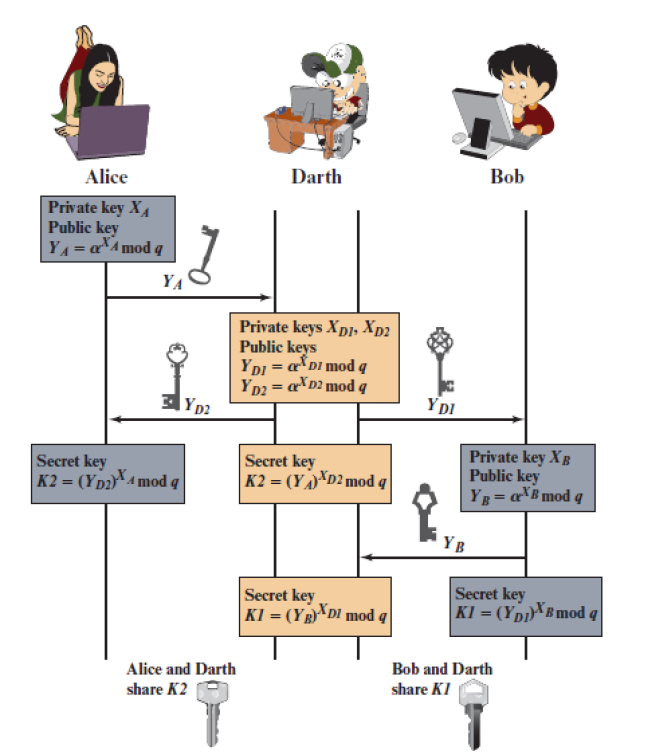
\includegraphics[width=0.5\textwidth]{resources/MITM-Diffie-Hellman.png}
    \captionof{figure}{Ataque Man-in-the-Middle en Diffie--Hellman}
\end{center}

\subsection{DSS}

\textbf{Digital Signature Standard (DSS):}
\begin{itemize}
    \item Utiliza el algoritmo de firma digital junto con \textbf{SHA-1}.
    \item No puede emplearse para \textbf{cifrado} ni para \textbf{intercambio de claves}, únicamente para \textbf{firma digital}.
\end{itemize}

\subsection{ECC}

\textbf{Elliptic Curve Cryptography (ECC):}
\begin{itemize}
    \item Similar a \textbf{RSA}, pero funciona con claves más pequeñas.
    \item Ofrece un nivel de confianza algo menor que RSA.
    \item Basado en el \textbf{problema de la curva elíptica}.
\end{itemize}



\section{Firmas digitales}

Una \emph{firma digital} es un patrón de bits dependiente de los datos, generado por un agente en función de un archivo o mensaje. Su propósito es garantizar la autenticidad, integridad y no repudio de la información firmada.

\subsection{Algoritmos de firma digital}
Entre los algoritmos más utilizados se encuentran:
\begin{itemize}
    \item DSA (Digital Signature Algorithm)
    \item RSA (Rivest–Shamir–Adleman)
    \item ECDSA (Elliptic Curve Digital Signature Algorithm)
\end{itemize}

\subsection{Elementos esenciales del proceso de firma digital}
El proceso de firma digital consta de los siguientes pasos:
\begin{enumerate}
    \item Se calcula un \textbf{resumen} (hash) del documento mediante una función hash segura.
    \item El firmante aplica su \textbf{clave privada} sobre el hash mediante el algoritmo de firma, generando la firma digital.
    \item Se envía el documento junto con la firma.
    \item El receptor calcula nuevamente el hash y utiliza la \textbf{clave pública} del firmante para verificar la validez de la firma.
\end{enumerate}

\subsection{Propiedades de la firma digital}
\begin{itemize}
    \item Verifica la identidad del autor y la fecha/hora de la firma.
    \item Autentica el contenido en el momento de la firma.
    \item Permite la verificación por terceros en caso de disputa.
\end{itemize}

\subsection{Ataques}
\begin{description}
    \item[Key-only attack:] El atacante solo conoce la clave pública.
    \item[Known message attack:] El atacante conoce varios pares (mensaje, firma).
    \item[Generic chosen message attack:] El atacante elige una lista de mensajes independientemente de la clave pública de A y obtiene de A firmas válidas para esos mensajes.
    \item[Directed chosen message attack:] Igual que el anterior, pero el atacante elige los mensajes en función de la clave pública de A.
\end{description}

\subsection{Falsificación}
\begin{itemize}
    \item \textbf{Total break:} El atacante obtiene la clave privada y puede generar firmas válidas para cualquier mensaje.
    \item \textbf{Universal forgery:} El atacante genera firmas válidas para cualquier mensaje sin conocer la clave privada.
    \item \textbf{Selective forgery:} El atacante falsifica una firma válida para un mensaje específico.
    \item \textbf{Existential forgery:} El atacante genera al menos una firma válida para algún mensaje (aunque no tenga sentido práctico).
\end{itemize}

\subsection{Certificado de clave pública}
\begin{figure}[h!]
    \centering
    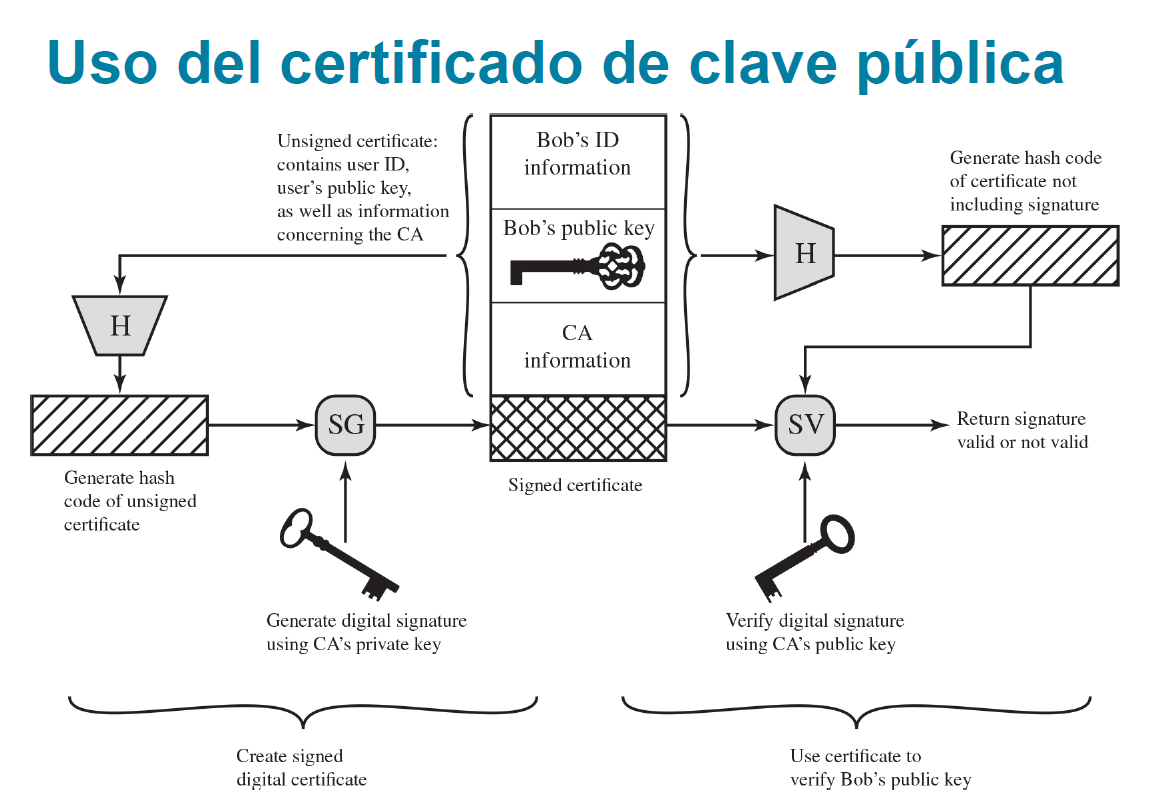
\includegraphics[width=0.75\textwidth]{resources/PublicKey_CA.png}
    \caption{Certificado de clave pública emitido por una Autoridad de Certificación (CA).}
\end{figure}

El certificado de clave pública contiene:
\begin{itemize}
    \item Información del propietario.
    \item La clave pública.
    \item Información de la CA (por ejemplo, en España la FNMT).
    \item La firma digital de la CA.
\end{itemize}

\subsection{Sobres digitales}

Un \emph{sobre digital} combina cifrado simétrico y asimétrico para proteger un mensaje.
El emisor genera una \textbf{clave simétrica aleatoria} para cifrar el mensaje y luego cifra dicha clave con la \textbf{clave pública del receptor}.
Ambos elementos (mensaje cifrado y clave cifrada) forman el sobre digital.
El receptor usa su \textbf{clave privada} para recuperar la clave simétrica y descifrar el mensaje.

\begin{center}
    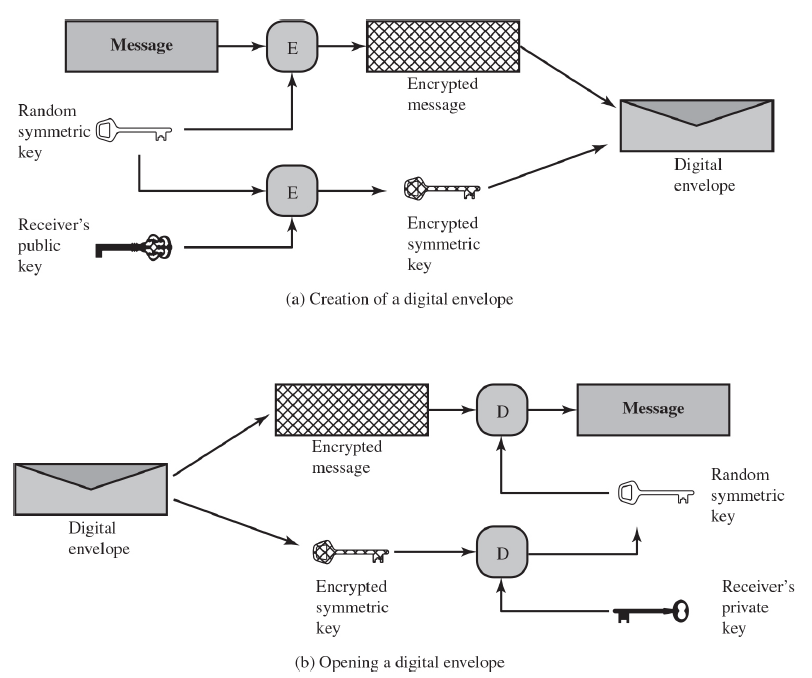
\includegraphics[width=0.65\textwidth]{resources/DigitalEnvelopes.png}
    \captionof{figure}{Esquema de un sobre digital}
\end{center}

\section{Números aleatorios}

\subsection{Aleatorios vs. Pseudoaleatorios}

Los \textbf{números aleatorios} son impredecibles y no siguen un patrón, mientras que los \textbf{números pseudoaleatorios} son generados por algoritmos deterministas y pueden reproducirse si se conoce la semilla inicial.

Aun así, los números pseudoaleatorios pueden considerarse impredecibles si la \textbf{fuente de entropía} utilizada (por ejemplo, radiación o ruido térmico) proviene de un fenómeno natural. (TRNG) True Random Number Generator

\subsection{Propiedades de los números aleatorios}

\begin{itemize}
    \item \textbf{Uniformidad:} cada valor dentro del rango tiene la misma probabilidad de ser seleccionado.
    \item \textbf{Independencia:} la aparición de un número no afecta la aparición de los demás.
    \item \textbf{No repetición:} en una secuencia dada, los números no deben repetirse.
    \item \textbf{Impredecibilidad:} es imposible anticipar el siguiente número en la secuencia basándose en los anteriores.
\end{itemize}

\end{document}
